%%
%
% En algunas distribuciones es necesario instalar el paquete texlive-publishers
%
%\documentclass[letterpaper,aps,twocolumn,pre,nofootinbib]{revtex4}
%\documentclass[twocolumn]{article}
\documentclass[conference]{IEEEtran}

\usepackage[spanish]{babel}
\usepackage{amsmath,amssymb,amsfonts,amsthm}
\usepackage{graphicx}
%\usepackage{bbm}
\usepackage[utf8]{inputenc} % Caracteres en Español (Acentos, ñs)
\usepackage{url} % ACENTOS
\usepackage{hyperref} % Referencias
\usepackage{subfig}
\usepackage{lipsum}
\usepackage{balance}


%%%%%%%%%%%%%%%%%%%%%%%%%%%%%%%%%%%%%%%%%%%%%
% PARCHE PARA ELIMINAR LA FECHA DEL DOCUMENTO
% 
\usepackage{etoolbox}
\makeatletter
% \frontmatter@RRAP@format is responsible for the parentheses
\patchcmd{\frontmatter@RRAP@format}{(}{}{}{}
\patchcmd{\frontmatter@RRAP@format}{)}{}{}{}
%\renewcommand\Dated@name{}
\makeatother	
% FIN DEL PARCHE
% 
%%%%%%%%%%%%%%%%%%%%%%%%%%%%%%%%%%%%%%%%%%%%%

%%%%%%%%%%%%%%%%%%%%%%%%%%%%%%%%%%%%%%%%%%%%%
% PARCHE PARA PERMIRIR UTILIZAR BIBLATEX EN ESTA PANTLLA
%\PassOptionsToPackage{square,numbers}{natbib}
%\RequirePackage{natbib}  
%%%%%%%%%%%%%%%%%%%%%%%%%%%%%%%%%%%%%%%%%%%%%

%\usepackage[backend=bibtex,sorting=none]{biblatex}
% Estas lineas permiten romper los hipervinculos muy largos !!!!
%\setcounter{biburllcpenalty}{7000}
%\setcounter{biburlucpenalty}{8000}
%\addbibresource{references.bib}

% Actualiza en automático la fecha de las citas de internet a la fecha de la compilación del documento
\usepackage{datetime}
\newdateformat{specialdate}{\twodigit{\THEDAY}-\twodigit{\THEMONTH}-\THEYEAR}
\date{\specialdate\today}

% la sentencia \burl en las citas... 
\usepackage[hyphenbreaks]{breakurl}

\renewcommand\spanishtablename{Tabla}
\renewcommand\spanishfigurename{Figura}

%\usepackage{datetime}
%\newdateformat{specialdate}{\twodigit{\THEDAY}-\twodigit{\THEMONTH}-\THEYEAR}
%\newdateformat{specialdate}{\twodigit{\THEDAY}-\THEYEAR}
%\date{\specialdate\today}


\begin{document}
%%%%%%%%%%%%%%%%%%%%%%%%%%%%%%%%%%%%%%%%%%%%%
% Definitions
%
%
% Define your special symbols here
%
%%%%%%%%%%%%%%%%%%%%%%%%%%%%%%%%%%%%%%%%%%%%%

% use to set width of figures
\newcommand{\breite}{0.9} %  for twocolumn
\newcommand{\RelacionFiguradoscolumnas}{0.9}
\newcommand{\RelacionFiguradoscolumnasPuntoCinco}{0.45}


%%%%%%%%%%%%%%%%%%%%%%%%%%%%%%%%%%%%%%%%%%%%%
% End Definitions
%%%%%%%%%%%%%%%%%%%%%%%%%%%%%%%%%%%%%%%%%%%%%


%Title of paper
\title{Reporte de Proyecto Individual 1 \\ Tabla periodica moderna}

% Trabajo Individual
\author{\IEEEauthorblockN{Kevin Alejandro Hernandez Campillo\IEEEauthorrefmark{1}}
\IEEEauthorblockA{\IEEEauthorrefmark{1}Ingeniería en Tecnologías de la Información\\
Universidad Politécnica de Victoria}
}


%\date{}

\maketitle

\begin{abstract} 
La problemática a resolver consiste en crear un programa que simule una tabla periódica, donde se puedan guardar elementos y leerlos aparir de un archivo guardado en el disco duro. En este trabajo se propone una solución creando un programa en el lenguaje de programación Python3 y siguiendo el paradigma orientado a objetos. Para esto se crearon dos métodos principales que realizan estas dos acciones a partir de las distintas opciones que nos da el método open. Como resultado se tiene un programa capaz de añadir nuevos elementos al fichero y de obtener inflacionario acerca de estos elementos a partir de un parámetro de búsqueda.

\end{abstract}


%\maketitle must follow title, authors, abstract, \pacs, and \keywords




\section{Introducción}

En el presente trabajo se desarrollo el proyecto titulado 'Tabla periódica moderna', el cual consta de un programa de interfaz de linea de comandos(CLI), que realiza dos acciones principales: Añadir nuevos elementos guardándolos en un archivo y leer los elementos existentes en el registro por medio de opciones de búsqueda, para una mejor descripción del proyecto consultar la sección Desarrollo Experimental. Para esto se utilizo el lenguaje de programación Python3 y el paradigma de programación orientado a objetos(POO).
 
\section{Desarrollo Experimental}

En primera instancia se consulto la liga proporcionada por el profesor \cite{MTP}, para así poder determinar la naturaleza del problema, con esto se determino que el proyecto debe consistir en una programa de CLI que nos permita realizar dos funciones principales, añadir nuevos elementos y explorar los elementos registrados. Los elementos añadidos deben registrarse en un archivo en el disco duro, y se debe almacenar el nombre del elemento, el símbolo, el numero atómico, el pero atómico y un breve comentario sobre del elemento. La exploración de los elementos debe realizarse con respecto a la opción que elija el usuario, pudiendo ser buscar por nombre, por símbolo, por numero atómico, o por peso atómico.\par

Para iniciar se realizo una breve investigación sobre la tabla periódica para determinar que tipos de datos almacena\cite{NGE}. Posteriormente, se investigo la implementación del paradigma orientado a objetos en Python\cite{gitPOO}\cite{IP}. Tras esto, se decidió dividir el programa tomando en cuenta las dos funciones principales, añadir elementos y explorar.

\subsection{Método add}
Como primer acercamiento a esta función se decidió simplificar el problema de tal modo que primero se investigo como trabajar con archivos en Python\cite{AP}, ya que para este método es imprescindible poder escribir en un fichero. Como resultado se escribió una primera version del método, dentro de la clase table, que solamente creaba un archivo con extenuación .txt, para esto se uso el método open, pasando como parámetros el nombre del archivo a crear y el modo, siendo en este caso el modo escritura(w), y posteriormente se pide al usuario que ingrese los datos previamente mencionados, estos datos eran almacenados en variables locales al método, todas de tipo String. Una vez que la información era ingresada, el programa daba un formato adecuado para que la información pudiese ser guardada de tal forma que simulaba una tabla\cite{Redhat}, esto generaba un String con todos los datos del elemento. Ahora para escribir los datos en el archivo creado usamos el método write. Con esto se consiguió que el elemento ingresado se almacenara en el fichero, pero surgía una problemática, al querer registrar un nuevo elemento el anterior se eliminaba.\par

Para corregir este inconveniente se estudio los modos de apertura que tiene el método open para trabajar con archivos\cite{docPy}, como resultado se concluyo que el mejor candidato era la opción append(a), la cual permite adjuntar el string pasado por el método wirte al fichero, y de esta forma no eliminar el contenido previamente guardado. Para finalizar se edito el formato de guardado para que el ultimo carácter del String de cada elemento fuera una secuencia de escape de nueva linea, de esta forma cada elemento seria guardado en una linea diferente en el fichero y los atributos del elemento serian separados por coma, obteniendo así un programa capaz de crear un archivo, si es que este no existiese ya, pedir los datos al usuario y escribir los datos ingresados con un formato especial.\par

Ya con esta primera version del método add se depuro el esta sección, para así prever cualquier error y darle una estética mas acorde al problema planteado.\par
 
El primer error lógico que se detecto fue aquel que se produce cuando se ingresan dos elementos con el mismo símbolo, nombre, numero o peso atómico, esto seria un error, ya que no existen dos elementos con estos atributos iguales. Obviamente se omitió comprobar si los comentarios eran iguales ya que esta información no es relevante para identificar a un elemento. Para corregir este error se creo un método que comprueba si existen dos elementos con cualquiera de estos atributos iguales, este método esta dentro de la clase Utilites y es llamado data\_exist, recibe como parámetros el nombre, símbolo, numero y peso atómico, si es que en el fichero existe un registro con alguno de esto atributos iguales, entonces este retorna Ture, de lo contrario False, esto se usa dentro del método add para verificar lo anteriormente mencionado, entonces de ser el caso en que ya existe un registro similar, no se instancia el archivo de registro y no se almacena la nueva información, y solo se muestra un mensaje que indica la existencia de los datos dentro del registro, para después retornar al menú principal. 

\subsection{Método explore}
Para este método es necesario leer el contenido del archivo, así que primero se consulto que opción del método open seria útil, dando como resultado que la opción indicada seria read(r), así que se procedió a escribir el método.\par 
En primer lugar el método pide al usuario que ingrese un numero del uno al cuatro, donde la primera opción seria buscar por nombre, la segunda opción por símbolo, la tercera por numero atómico y la ultima por peso atómico. Si la opción fuera correcta entonces se llama a un método parte de la clase utilities, llamado separate\_items, este método crea un objeto con el contenido del archivo creado usando la opción r del método open, y posteriormente usando el método readlines, se crea una lista con el contenido del archivo de tal modo que cada linea corresponde a un elemento de la lista. Una vez teniendo la información en una lista entonces se separan los atributos de cada elemento de tal forma que terminamos con una lista que contiene una lista por cada elemento, teniendo la información separada de esta forma es retorna la lista por el método. 

Ahora dependiendo de que opción de búsqueda se selecciono, se pide al usuario que ingrese el patrón de búsqueda, y se almacena en una variable llamada InputData. Posteriormente, dentro de un ciclo for se recorre la lista de elementos y por cada elemento se verifica un campo dependiendo de la opción seleccionada, es decir si se eligió buscar por nombre, entonces se busca usando [i][1] donde i es el iterador del for y 1 corresponde al campo del nombre del elemento, ya que dentro de la lista el index uno pertenece al nombre, el dos al símbolo, el tres al numero atómico y el cuarto al peso atómico, este valor se compara por cada elemento con el parámetro de búsqueda ingresado, almacenado en la variable InputData. Una vez encontrada una coincidencia, se imprime la información del elemento tomando en cuanta el valor del iterador i donde se encontrado el elemento buscado, en caso de que algún atributo no contenga ningun valor entonces se imprime Empty.

Por ultimo, en caso de que no se encontrara ninguna coincidencia entonces se imprime Data not found, para indicar al usuario que no se encontró ningún elemento con el parámetro de búsqueda ingresado.

\section{Resultados}
En las figuras siguientes se muestra una serie de capturas de pantalla del programa resultante. En primer lugar la figura \ref{img:01} muestra el menú principal del programa, donde el usuario puede seleccionar la tarea que desea realizar. A continuación, la figura \ref{img:02} muestra el funcionamiento del método add, donde el usuario añadió el elemento Potasio con todos sus atributos dando como resultado el registro de los datos en el registro. La figura \ref{img:03} muestra las diferentes opciones de búsqueda para la opción de explorar, pudiendo seleccionar por nombre, por símbolo, por numero atómico o por peso atómico. Por ultimo la figura \ref{img:04} muestra el resultado de seleccionar la opción de búsqueda 2 e ingresar el símbolo atómico H.\par




\begin{figure}[h!]
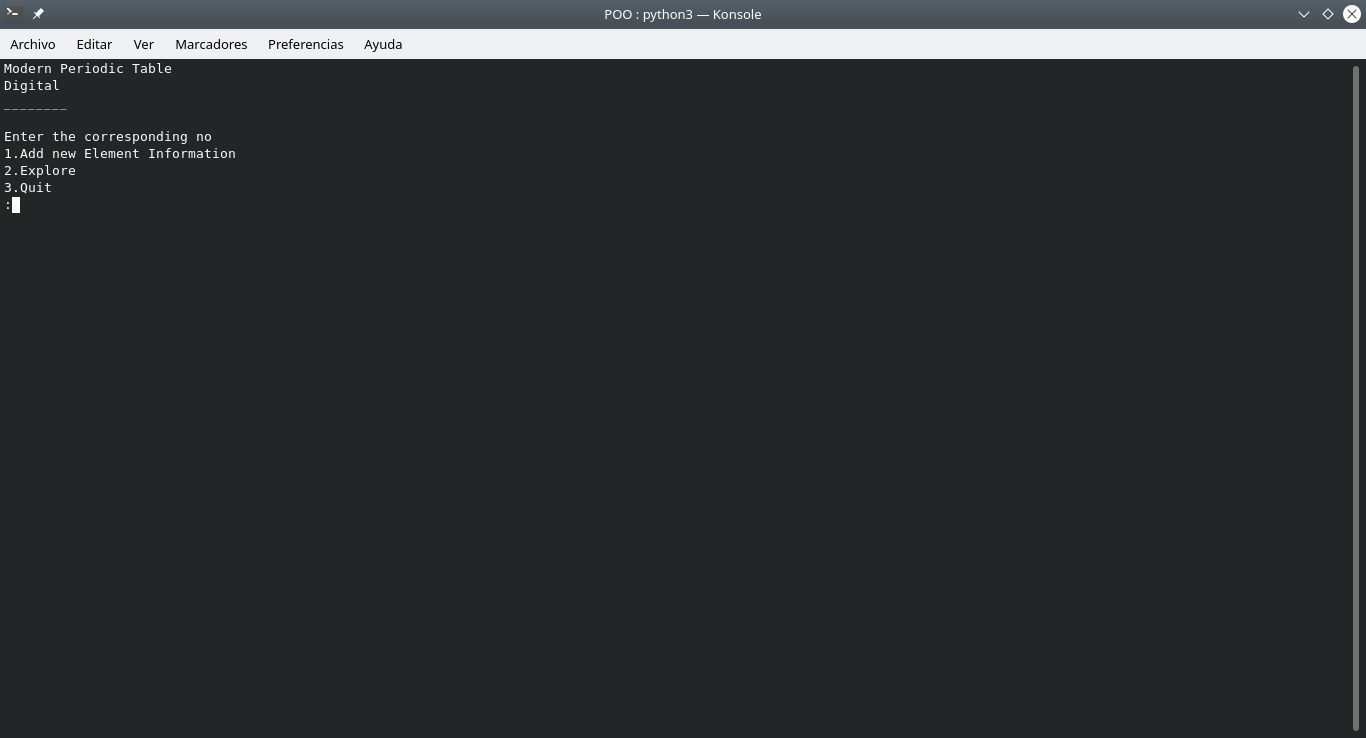
\includegraphics[width=1 \columnwidth]{cap_01.png}
\caption{Menú principal}
\label{img:01}
\end{figure}

\begin{figure}[h!]
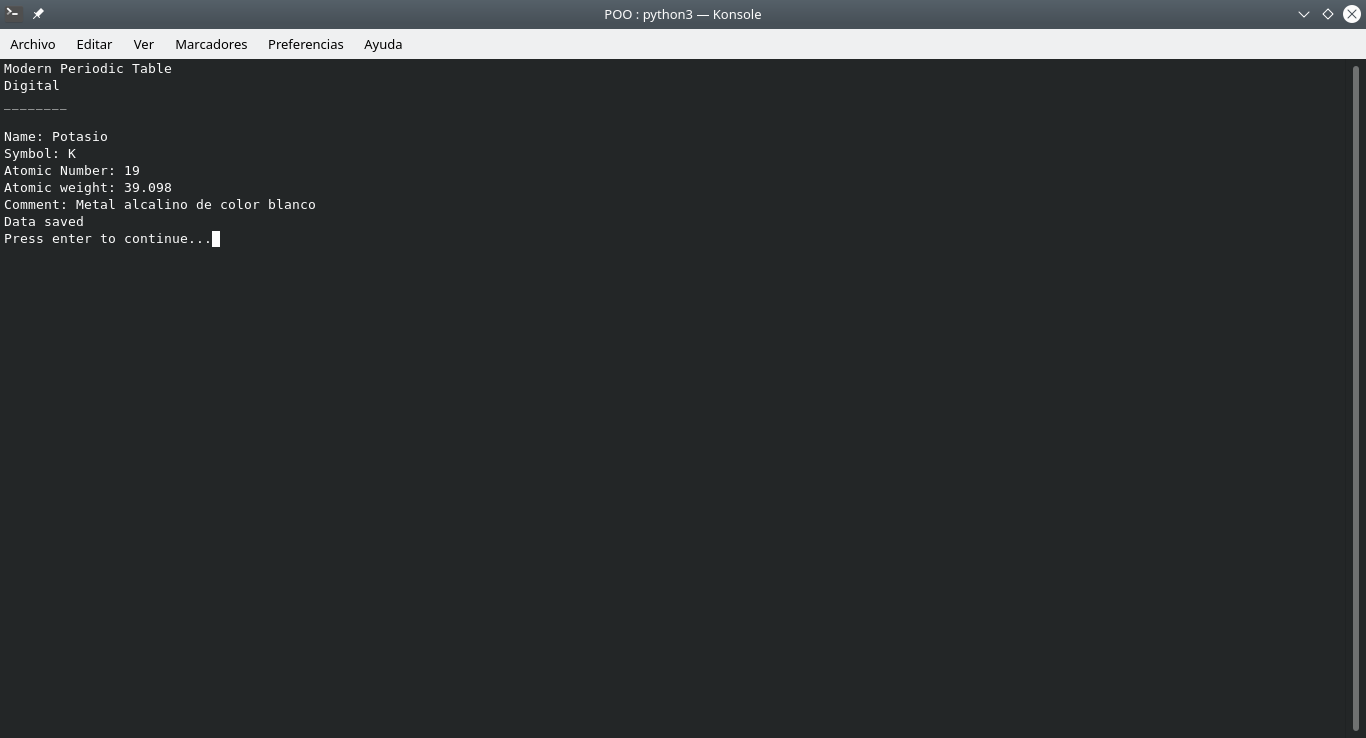
\includegraphics[width=1 \columnwidth]{cap_02.png}
\caption{Añadiendo elemento nuevo}
\label{img:02}
\end{figure}


%\subfloat[Menú principal]{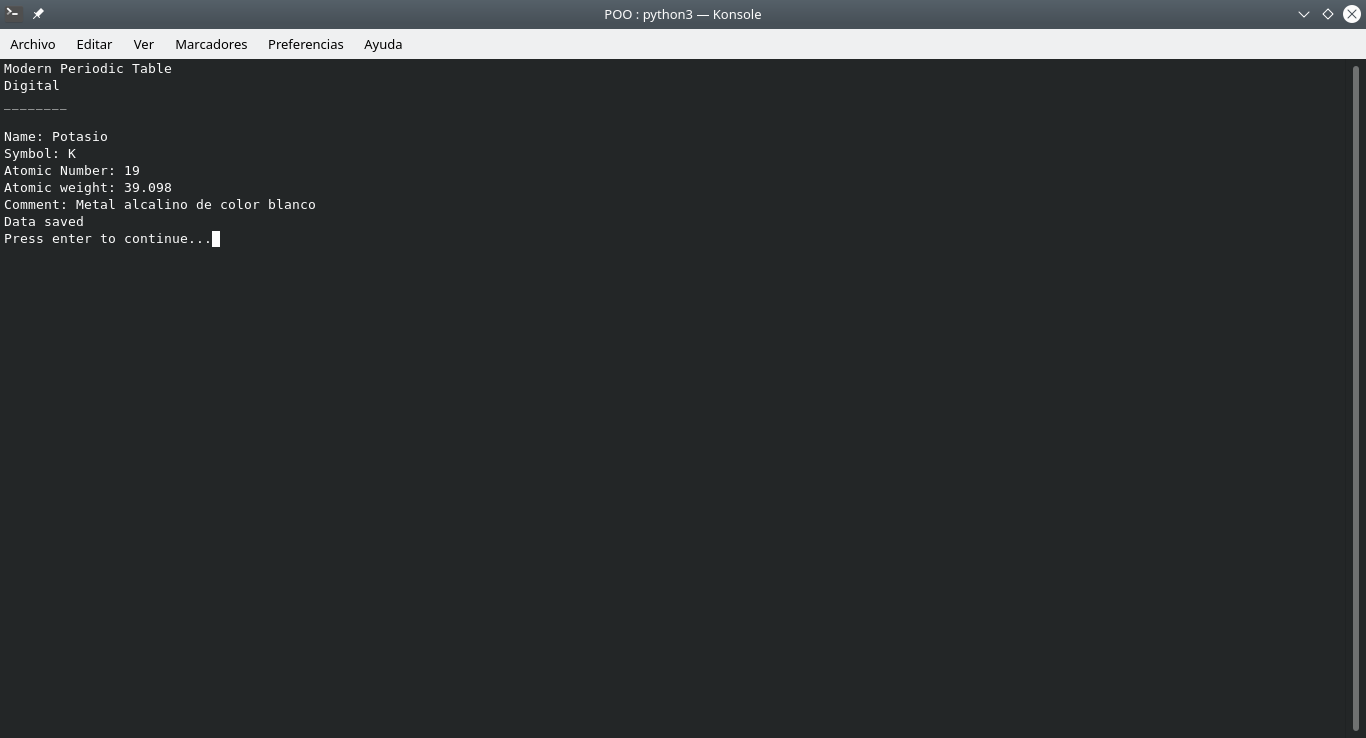
\includegraphics[width=0.5 \columnwidth]{cap_02.png}}\\
%\subfloat[Menú principal]{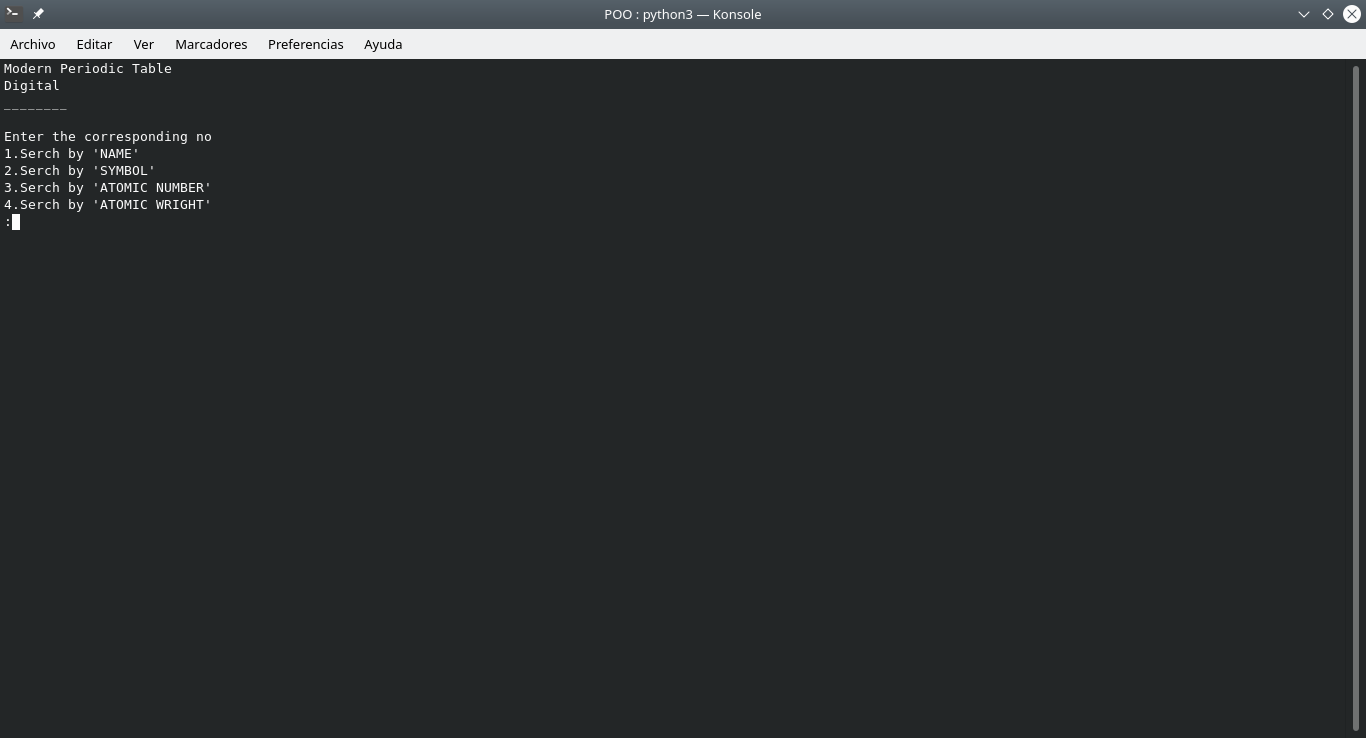
\includegraphics[width=0.5 \columnwidth]{cap_03.png}}

%\subfloat[Menú principal]{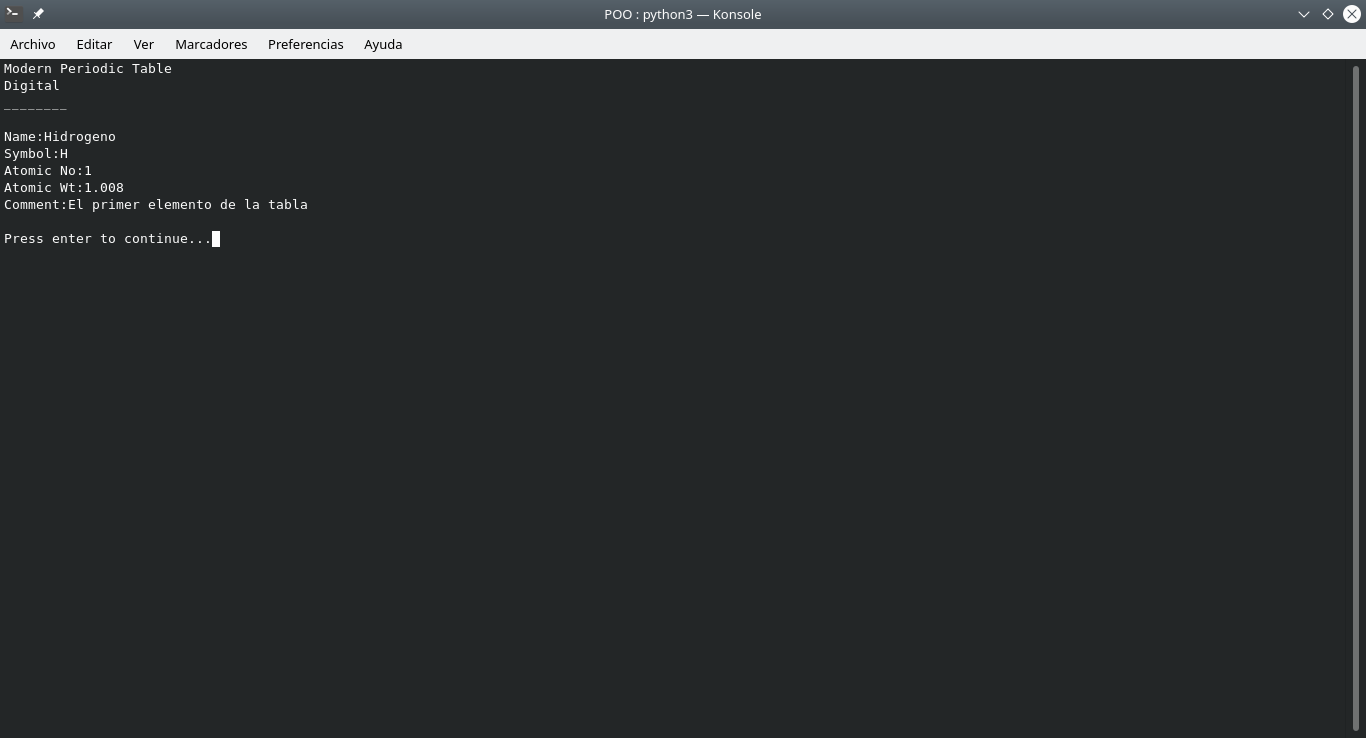
\includegraphics[width=0.5 \columnwidth]{cap_04.png}}
%\caption{Capturas de los diferentes menús del programa}


\section{Conclusión}
En el presente trabajo se desarrollo el proyecto titulado tabla periódica moderna, para el cual se implemento el lenguaje de programación Python3 y el paradigma de programación orientado a objetos. Ademas, se consultaron distintas fuentes\cite{proPy} para tomar como referencia los métodos de manejo de archivos con Python. A partir de la información recopilada se propuso una solución propia para el problema, dando como resultado un programa que es capas de añadir nuevos elementos en un archivo y buscar elementos en este archivo según el parámetro de búsqueda ingresado.

\begin{figure}[h!]
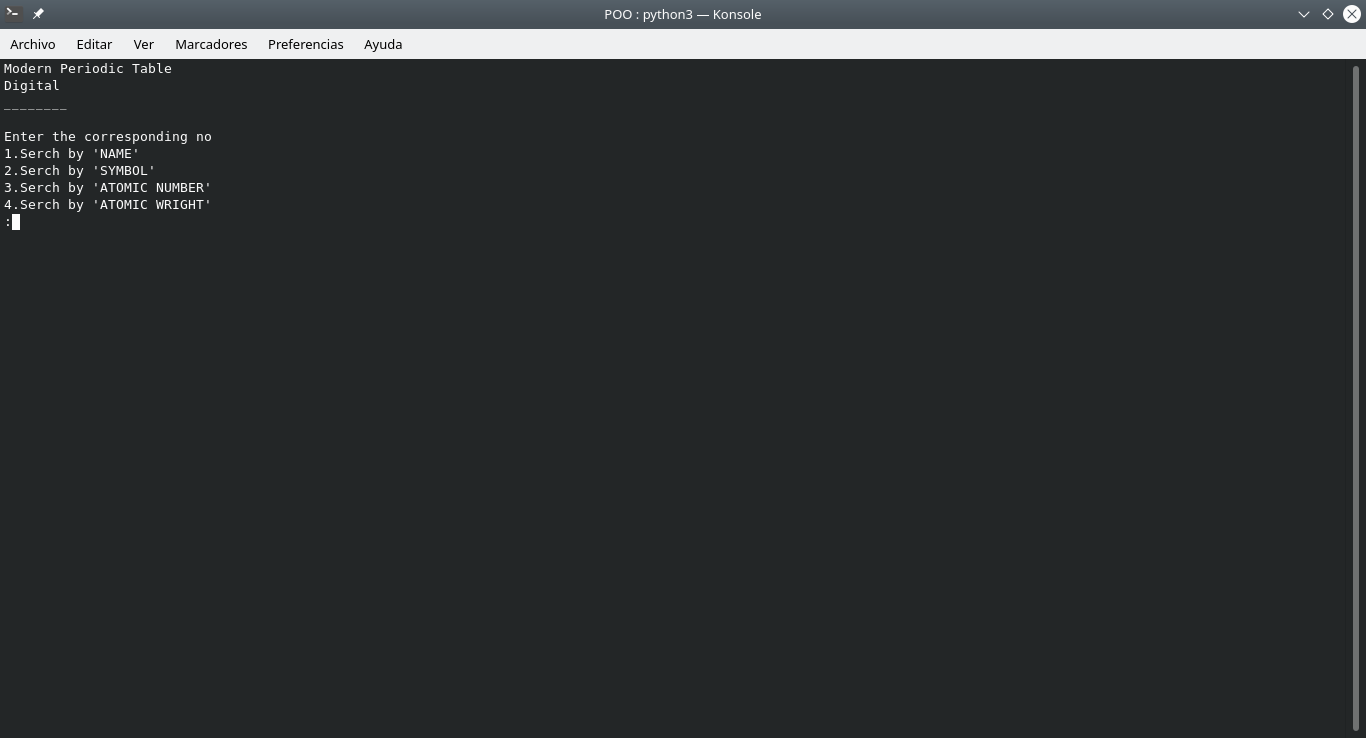
\includegraphics[width=1 \columnwidth]{cap_03.png}
\caption{Opciones de búsqueda}
\label{img:03}
\end{figure}

\begin{figure}[h!]
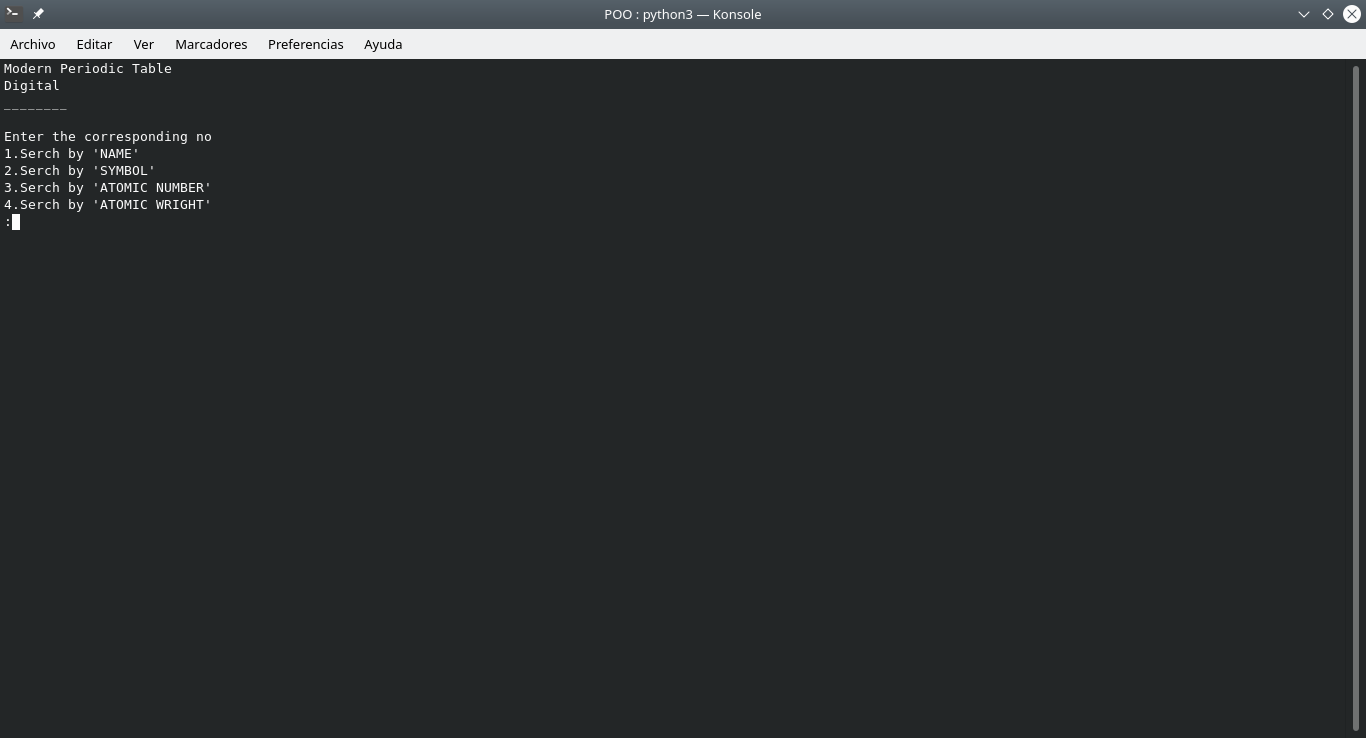
\includegraphics[width=1 \columnwidth]{cap_03.png}
\caption{Resultado al buscar por la opción dos el parámetro de búsqueda H}
\label{img:04}
\end{figure}

\newpage
\begin{thebibliography}{0}
	\bibitem{MTP} Rajendra Bohara. Modern Periodic Table C Project.\url{https://www.codewithc.com/modern-periodic-table-c-project/} Consultado el \today.
	\bibitem {NGE} Javier Flores, Gabriel Pinto. La tabla periódica, la forma de ordenar los elementos químicos. \url{https://www.nationalgeographic.com.es/ciencia/tabla-periodica-forma-ordenar-elementos-quimicos_15988} Consultado el \today.
	
	\bibitem {gitPOO} Megan Amendola, Juliano Garcia, Arda Kosar. OOP for beginners. \url{https://github.com/MissMeg/oop-for-beginners}Consultado el \today.
	
	\bibitem {IP} Carmen Graciani, José Ruiz. Introducción a python3. Tema 3: Programación orientada a objetos. \url{https://www.cartagena99.com/recursos/alumnos/apuntes/211007100920-Tema\%203.pdf} Consultado el \today.
en Python 

	\bibitem {AP} Bala Priya. Cómo manejar archivos en Python. \url{https://geekflare.com/es/manejar-archivos-en-python/} Consultado el \today.
	 
	 \bibitem {Redhat} ¿Almacenamiento de archivos, almacenamiento de bloques o almacenamiento de objetos? Redhat.com. \url{https://www.redhat.com/es/topics/data-storage/file-block-object-storage} Consultado el \today.

	\bibitem {docPy} Built-in Functions — Python 3.10.7 documentation.Python.org. \url{https://docs.python.org/3/library/functions.html} Consultado el \today.

	\bibitem {proPy} Abder Rahman. File Handling in Python. \url{https://code.tutsplus.com/tutorials/file-handling-in-python--cms-25623} Consultado el \today.

\end{thebibliography}


\end{document}













